\documentclass[12pt,pdftex,a4paper]{article}
\usepackage[english]{babel}
\usepackage{amsmath}
\usepackage{amssymb}
\usepackage{bbm}
\newcommand{\bbN}{\mathbbm{N}}
\newcommand{\bbR}{\mathbbm{R}}
\newcommand{\bbZ}{\mathbbm{Z}}
\newcommand{\bbI}{\mathbbm{I}}
\usepackage[pdftex]{graphicx}
\usepackage{listings}
\lstset{language=Python,basicstyle=\footnotesize}
\begin{document}
\title{Practical Course Robotics\\Weekly Summary}
\author{Mohammed Muddasser, Raphael Broesamle}
\date{Calendar week 28}
\maketitle
%%%%%%%%%%%%%%%%%%%%%%%%%%%%%%%%%%%%%%%%%%%%%%%%

\section*{Achievements this week}
\begin{itemize}
\item
Work Package 4 - Goalie:
The objectives to move the goalie to the desired position after the throw have been integrated and synchronized in the environment.

\item
Work Package 5 - Integration and Extensive Testing:
Integration of all work-packages complete. Synchronization between and throw and block is accomplished.
\\
\begin{enumerate}
    \begin{minipage}{\linewidth}
        \centering
        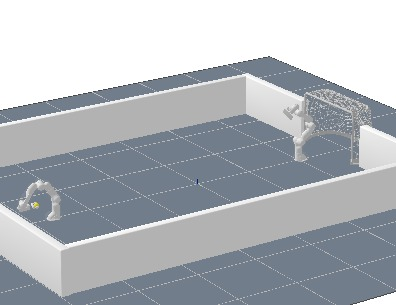
\includegraphics[width=.3\textwidth]{pos1.jpeg}
        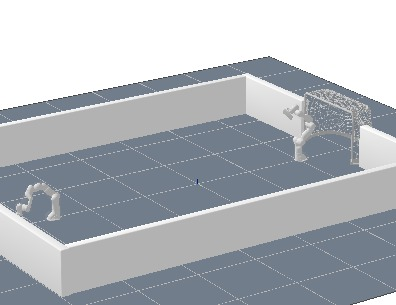
\includegraphics[width=.3\textwidth]{pos2.jpeg}
        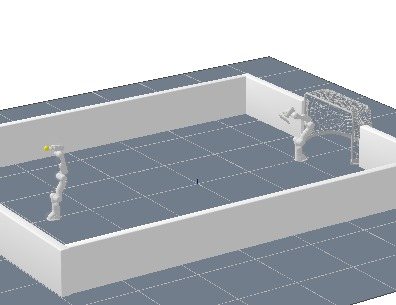
\includegraphics[width=.3\textwidth]{pos3.jpeg}
        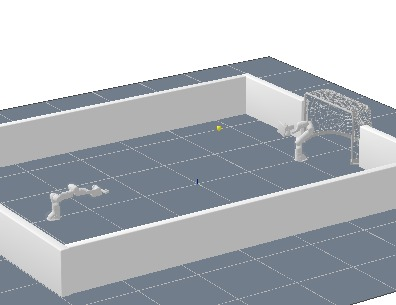
\includegraphics[width=.3\textwidth]{pos4.jpeg}
        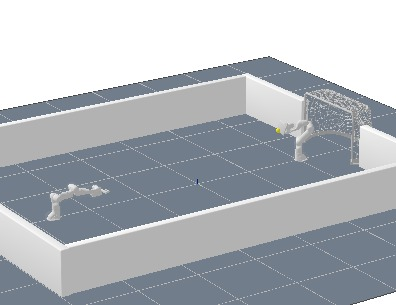
\includegraphics[width=.3\textwidth]{pos5.jpeg}
        \captionof{\\ Simulation snapshots of various positions taken with time }
    \end{minipage}
\end{enumerate}
\end{itemize}

\section*{Overall Status}
\begin{tabular}{ |p{10cm}||p{6cm}| }
 \hline
 \multicolumn{2}{|c|}{ \textbf{Overall Status}} \\
 \hline
\textbf{Work-package} & \textbf{Status} \\
 \hline
 Work Package 1: Scene creation                     & Done\\
 Work Package 2: Throwing the ball                  & Done\\
 Work Package 3: Ball Management                    & Done\\
 Work Package 4: Goalie - BlockBot                  & Done\\
 Work Package 5: Integration and Extensive Testing  & In Progress\\
 Work Package 6: Video and Presentation preparation & In Progress\\
 \hline
\end{tabular}

\section*{Goals for the final week}
\begin{itemize}
\item
Work Package 5 - Integration and Extensive Testing:
Fine tuning the optimization functions. Trying out throws and blocks from various directions.
\item
Work Package 6 - Video and Presentation preparation\end{itemize}

%%%%%%%%%%%%%%%%%%%%%%%%%%%%%%%%%%%%%%%%%%%%%%%%
\end{document}

